%------------------------------------------------------------------------------
% Template file for the submission of papers to IUCr journals in LaTeX2e
% using the iucr document class
% Copyright 1999-2003 International Union of Crystallography
% Version 1.2 (11 December 2002)
%------------------------------------------------------------------------------
%
\documentclass[preprint, pdf]{iucr}              % DO NOT DELETE THIS LINE
                   \def\href#1{\relax}\let\foo\caption
\ifPDF
  \RequirePackage{hyperref}
  \PassOptionsToPackage{pdftex,bookmarksopen,bookmarksnumbered}{hyperref}
  \voffset=-0.5in
\fi
\let\caption\foo

\usepackage{graphicx}
\usepackage[T1]{fontenc}
\usepackage[utf8]{inputenc}
%\usepackage{eps2pdf}

 \paperprodcode{a000000}      % Replace with production code if known
 \paperref{xx9999}            % Replace xx9999 with reference code if known
 \papertype{IU}               % Indicate type of article
 \paperlang{english}          % Can be english, french, german or russian
 \journalcode{J}             % Indicate the journal to which submitted
 \journalyr{2017}
 \journalreceived{\relax}
 \journalaccepted{\relax}
 \journalonline{\relax}

\begin{document}                  % DO NOT DELETE THIS LINE

\title{Calibration of experimetal setups with {pyFAI}: still detector or
moving detector}
\shorttitle{Using pyFAI with a goniometer}

 \author[a]{V.}{Valls}
 \cauthor[a]{J.}{Kieffer}{jerome.kieffer@esrf.eu}
 
 
 \aff[a]{ESRF, The European Synchrotron, CS40220, 38043 \city{Grenoble}
 Cedex 9, \country{France}}
 \shortauthor{Valls and Kieffer}


\keyword{Powder diffraction}
\keyword{translation table}
\keyword{goniometer}
\keyword{geometry calibration}



\maketitle                        % DO NOT DELETE THIS LINE

\begin{synopsis}
New tools to calibrate different types of scattering experiments : still
detectors or moving detectors.
\end{synopsis}

\begin{abstract}

According to an internal survey performed among the beam-line scientists at
the European Synchrotron (ESRF) in 2016, the factor limiting the users'
productivity at diffraction beamlines is the calibration of the experimental
setup before the access to the raw data for their reduction. 
This issue is curently worked-around by providing to the users the proper
geometry or even the reduced data, but this prevent the
re-processing in home institutes and also the re-interpretation of data which
is needed as part of the open-data initiative.

This contribution presents a couple of new calibration tools: 
a new graphical user interface for calibrating the detector position for a 
diffraction experiment performed with a fixed large area detector and a library
to be used in \textit{Jupyter notebook} for calibrating the move of the
detector on a gonimeter arm (or any other moving table) for perfoming
diffraction experiements with a moving detector.
\end{abstract}


\section{Introduction}

Area detectors mounted on goniometer arms are commonly available for
powder-diffraction data acquisition in lab-source diffractometer (for example
Rigaku HyPix-3000).
%The larger number of pixels trades-of the resolution for speed.
On the opposite, moving detector setups are rarely used at synchrotrons for
the data acquisition itself, even if most of the detectors are mounted on a
moving table or on a goniometer. 
One counter example may be \cite{Gao:kc5032} where the beamline is equiped with
a moving stip-detector (not an area detector).

So at large facilities like synchrotons, larger detectors are 
preferred and kept fix during the whole acquisition, often to ease the
data-reduction step.
The fixed position setup combined with the speed of modern detectors allows
easily the acquisition in kinetic mode for following chemical reaction or other
physical processes \cite{id15, id31}.
Even with fixed geometries, the determination of the detector's position is
still an issue for a majority of users, according to a survey conducted among 
the beam-lines scientists of the European Synchrotron (internal survey in 2016). 
Hence a new grephical user interface has been developped for pyFAI, focusing
on the user's experience to give them autonomy in data analysis, once back to the
home institutes.

High-Q diffraction signal acquisition is needed \cite{Chupas:wf5000} for
Pair-wise Distribution Function (PDF) analysis which requires very large
detectors and higher energies to be able to cover the Q-range with one single frame.
When speed is not a critical parameter, such experiment could be performed
with smaller detectors mounted on a moving arm, and moved in front of
the sample during the acquisition. 
This setup is indeed already available on most diffraction beam-lines as
detectors are often mounted either on a translation table or on a
goniometer. 
The new pyFAI module for dealing with goniomaters and their calibration is
presented in this contribution, with a couple of \textit{Jupyter Notebooks}
\cite{ipython} proposed as suplementary materials.

This document presents first shortly the pyFAI library \cite{fv5028} then how to
merge multiple diffraction images acquired at different positions with this
library \cite{PyFAI_PDJ}. 
After recalling how calibration works in pyFAI, this document then 
presents the new graphical user interface and how to
calibrate the absolute position of every single pixel in the detector when
mounted on a goniometer (or of the translation table) as function of the  motor
positions of the goniometer (assuming there are coupled with encoders). 

\section{The Python Fast Azimuthal Integration library (PyFAI)}

PyFAI is a Python \cite{python} library used to transform 2D diffraction images into
1D powder diffraction pattern using re-binning of the pixel position to polar coordinates.
It provides in addition tools to calibrate the detector position, i.e. determine
where it is located in space from the conics drawn by the Debye-Scherrer cones
intersected by the detector (ellipses when the detector is planar and slightly
inclined). This document describes the processing implemented in pyFAI
v0.14 which is to be published in fall 2017 and still under development.

Azimuthal integration is performed in two steps, the first is a pixel-wise
transformation corresponding the image correction:
$$
I_{cor} = \frac{signal}{normalization}  = \frac{I_{raw} - I_{dark}}{F \times
\Omega \times P \times A } $$
where $I_{raw}$ is the raw detector signal, $I_{dark}$ is the dark current
image (may be also the background image for certain experiments), $F$ refers to
the flat-field correction, $\Omega$ to the solid angle of the given pixel, $P$
refers to polarization correction and $A$ refers to detector efficiency due
to in volume absorption due to parallax effects.

For azimuthal integration the numerator of this formula, her-after referred as
\textit{signal}, is separated from the denominator which is referred as
\textit{normalization}.

The re-binning of the data is performed using an histogram of the position ($q$
or $2\theta$ values) weighted by the \textit{signal}.
This gives the sum of all signals withing a ring.
A second histogram of the positions is calculated, weighted by the
\textit{normalization} this time, which gives the sum of all normalization
values.

The average signal over a ring is then simply the ratio of the two histograms.

$$
<I>_{ring} = \frac{\sum\limits_{i \in ring} c_i \times signal_i}
                  {\sum\limits_{i \in ring} c_i \times normalization_i} 
$$

In this equation, the parameter $c_i$ correspond to the fraction of area of a
pixel falling into a specific bin. 
As pyFAI provides multiple pixel splitting schemes, the differ only by their
$c_i$ coefficients. 
Simple weighted histograms corresponds actually to no splitting at all; in this
case the parameter $c_i$ is 1 for pixels falling in the bin an 0 for all the
others.
  
Those multiple pixel splitting schemes have already been described in
 \cite{fv5028} and can be stored to accelerate the calculation of the
histogram  \cite{kieffer_ashiotis-proc-euroscipy-2014}.

\section{Azimuthal integration of multiple frames taken at multiple geometries}

The integration of multiple images taken at varying position has first been
reported for pyFAI in  \cite{PyFAI_PDJ}. 
The procedure is conceptually similar to the integration on a single image,
except that the various histograms, all performed on the same grid, are summed
together, signals from all images on the numerator and normalization from all
images on the denominator.

$$
<I>_{ring} = \frac{\sum\limits_{imges} \sum\limits_{i \in ring} c_i \times
signal_i} {\sum\limits_{imges} \sum\limits_{i \in ring} c_i \times
normalization_i} 
$$

The normalization for solid angle correction $\Omega$ has to be performed in
absolute solid-angle (unlike in single frame integration) as different
geometries may have very different sample-detector distances. 
This explains why a single image integrated in multi-geometry mode  has
intensity orders of magnitude larger than with the normal pyFAI integration
methods.

\section{Calibration of the detector position}

\subsection{Principle of the calibration using a Debye-Scherrer diffraction
image}
The calibration of a detector position is performed using the Debye-Scherrer
rings collected from a reference powder called \textit{calibrant}.
The rings are extracted automatically and control points are placed at the
local maxima on the rings.
The geometry of the experiment is obtained from a least squares fitting of
the $2\theta$ angles.
In this work we will call them ``rings'' even if, for planar detector,
they are actually the conic intersections of the X-ray beam cones
with the detector plane.
For non planar detectors detector (also supported by pyFAI) those ``rings'' can
be any type of curve.

The least squares refinement is performed on an internal parameter-set
containing six  parameters (or seven with the wavelength), defined around the
concept of Point Of Normal Incidence (hereafter named \textsc{poni}) which is
the orthogonal projection  of the sample position on the detector plan 
(or z=0 when the detector is non-planar and z varies from pixel to pixel).
This \textsc{poni} differs from the beam-center used in programs like
Fit2D \cite{fit2d} as the \textsc{poni} is always defined and often lies within
the detector's image, as the detector best works when facing the sample.

So the parameters refined are the following:
\begin{itemize}
  \item \textit{dist}: the distance in meter from the sample position to the
  \textsc{poni}
  \item \textit{poni1} and \textit{poni2}: coordinate of the
  \textsc{poni} in meter within the detector plan (z=0) along the slow and fast
  dimension of the detector image (usually the row number and the column
  number, i.e. ``y, x'').
  \item \textit{rot1}, \textit{rot2} and \textit{rot3} which correspond to the
  rotation, expressed in radians, of the detector placed at the proper
  distance of the sample, along the 3 axis of the laboratory. The detector is
  first rotated around the vertical axis (rot1), then around the horizontal axis
  (rot2) and finally around the incoming beam (rot3). 
  \textsc{poni}
\end{itemize}

This parameter-set allows the description of any detector position in space.
The drawback is that some parameters are correlated: 
\begin{itemize}
  \item \textit{dist-wavelength}: reducing the wavelength is equivalent to
  increase the distance unless the diffraction angle $2\theta$ is actually
  large. It is advised to fix one of the the two unless the data are good
  quality and the angles are large.
  \item \textit{rot1-poni2} and \textit{rot2-poni1} as a small rotation can be
  interpreted as a larger translation. Fixing one decreases the uncertainty of
  the other by 2 orders of magnitude.
\end{itemize}

Moreover the \textit{rot3} is never refined and stays at zero unless specified
differently.  This can be used to simulate the rotation of the
experimental setup azimuthally. It has not effect in most cases, except for the
polarization of the incident beam during the diffraction process, which is the
main anisotropic contribution to the signal.

The parameters of the calibration are saved in text-files with the ``.poni''
extension and contain simply the six geometrical parameters, the detector
definition and the wavelength. 
This file can subsequently be loaded into an \textit{azimuthal integrator}
object, ready to perform azimuthal integration.

\subsection{Graphical user interface}

A semi-graphical calibration tool has been available as part of pyFAI
\cite{fv5028} since the origin of the project but this tool was considered too
hard to use by the users (while well accepted among the beamline staff).
Following the survey performed among the beam-line scientists of the European
Synchrotron, a new fully graphical user interface was developped, on top of 
the PyQt5 library \cite{pyqt} with specific focus on the ease of use for the
first time users.
The calibration of the experimental setup based on Debye-Scherrer rings images 
occues in five steps:
\begin{itemize}
  \item Settings: select wavelength, calibrant and detector (Figure
  \ref{calib_1}),
  \item Mask: a tool to draw a mask on top of the image (Figure
  \ref{calib_2}),
  \item Peak-picking: select ring and assign them to ring-numbers (Figure
  \ref{calib_3}),
  \item Geometry fitting: refinement of calibration (Figure
  \ref{calib_4}), 
  \item Integration: provides 1D and 2D integration of the image (Figure
  \ref{calib_5}). 
\end{itemize}

Thanks to the \textit{silx} \cite{silx} project, which joins
forces around data analysis for X-ray data, this new graphical user interface
already from masking tools and HDF5 browsing widgets.
This new interface allows a simpler manual peak-picking,
and still allows automatic ring extraction, fitting of the geometry and export
of the regrouped data. 
This calibration tool exports the result as a \textsc{poni}-file and can
save the list of control points used  for the fitting of the geometry as
\textsc{npt}-file

\begin{figure}
\label{calib_1}
\begin{center}
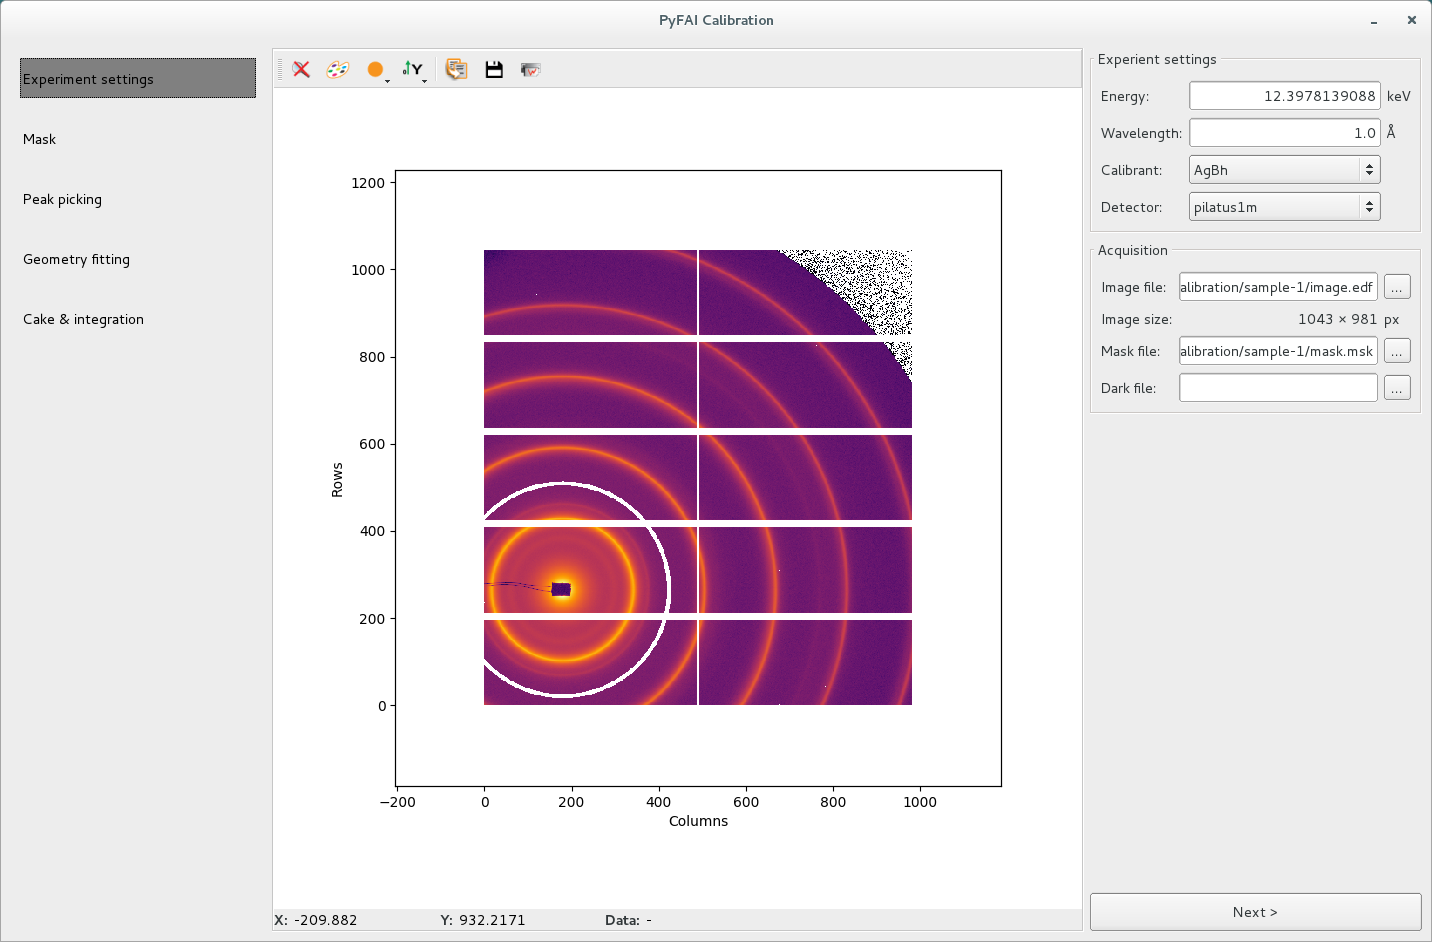
\includegraphics[width=9cm]{images/calibration-1-settings.png}
\caption{Setting up of the energy, calibrant and detector.}
\end{center}
\end{figure}
\begin{figure}
\label{calib_2}
\begin{center}
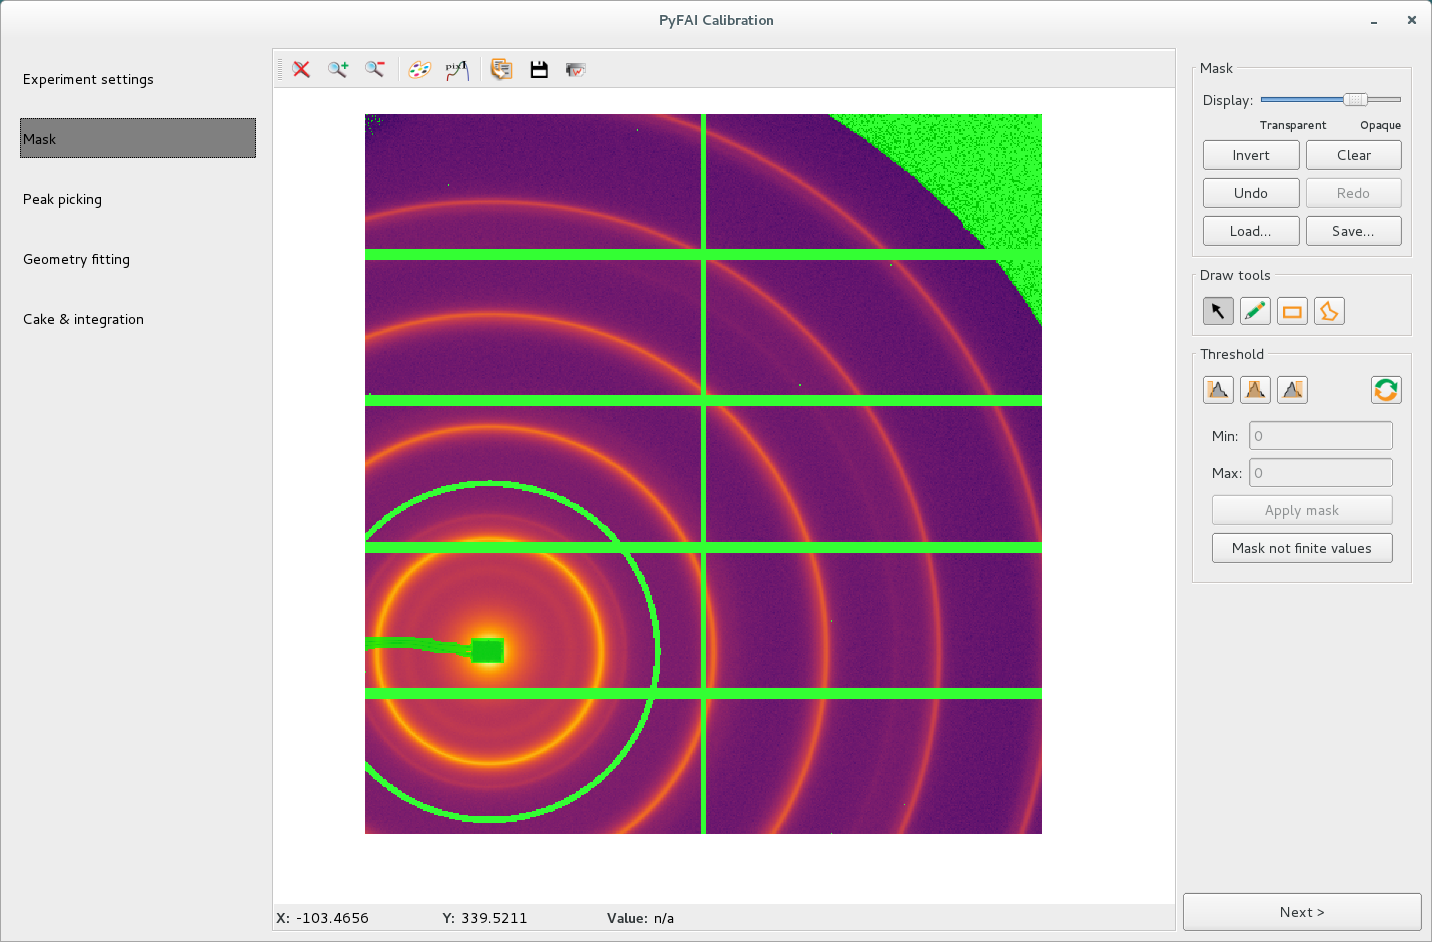
\includegraphics[width=9cm]{images/calibration-2-mask.png}
\caption{Integrated mask drawing tool}
\end{center}
\end{figure}
\begin{figure}
\label{calib_3}
\begin{center}
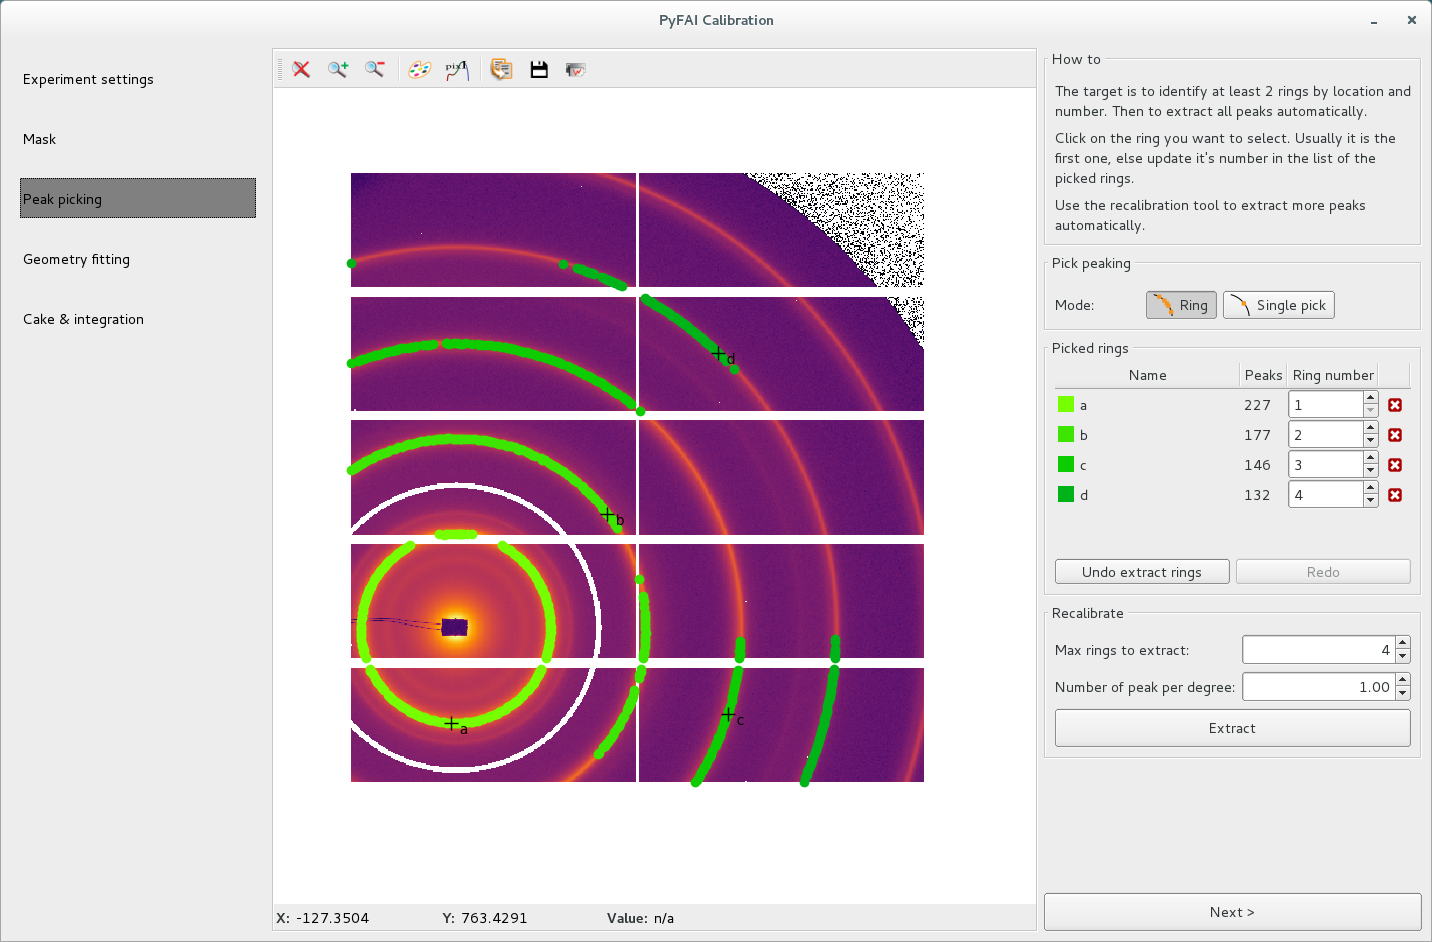
\includegraphics[width=9cm]{images/calibration-3-peak-picking.png}
\caption{Tool for peak-picking and ring assignment}
\end{center}
\end{figure}
\begin{figure}
\label{calib_4}
\begin{center}
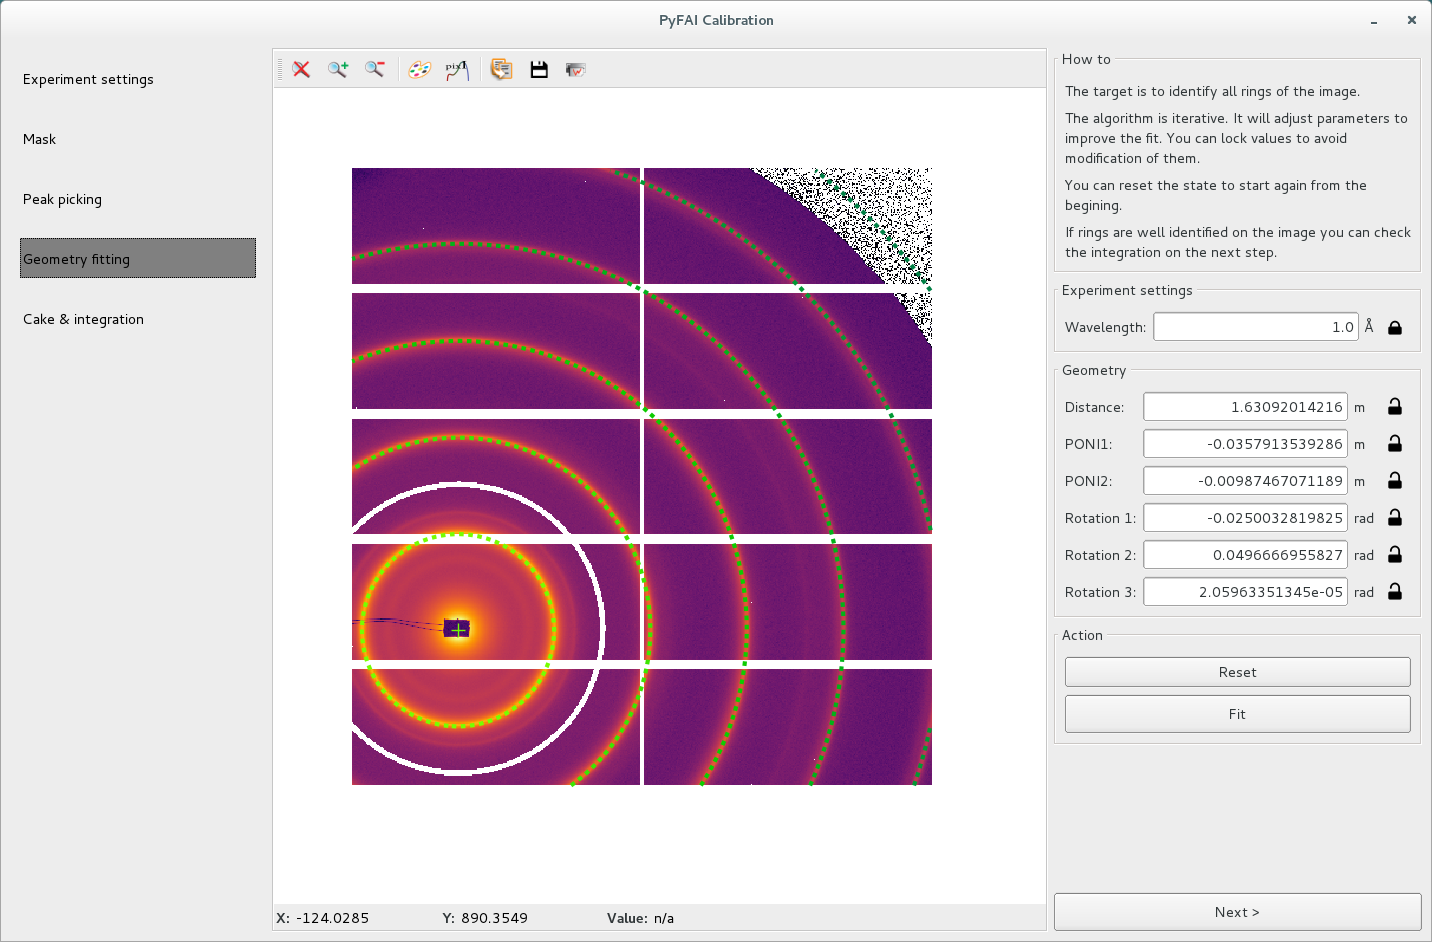
\includegraphics[width=9cm]{images/calibration-4-fitting.png}
\caption{Selection of the parameters to fit.}
\end{center}
\end{figure}
\begin{figure}
\label{calib_5}
\begin{center}
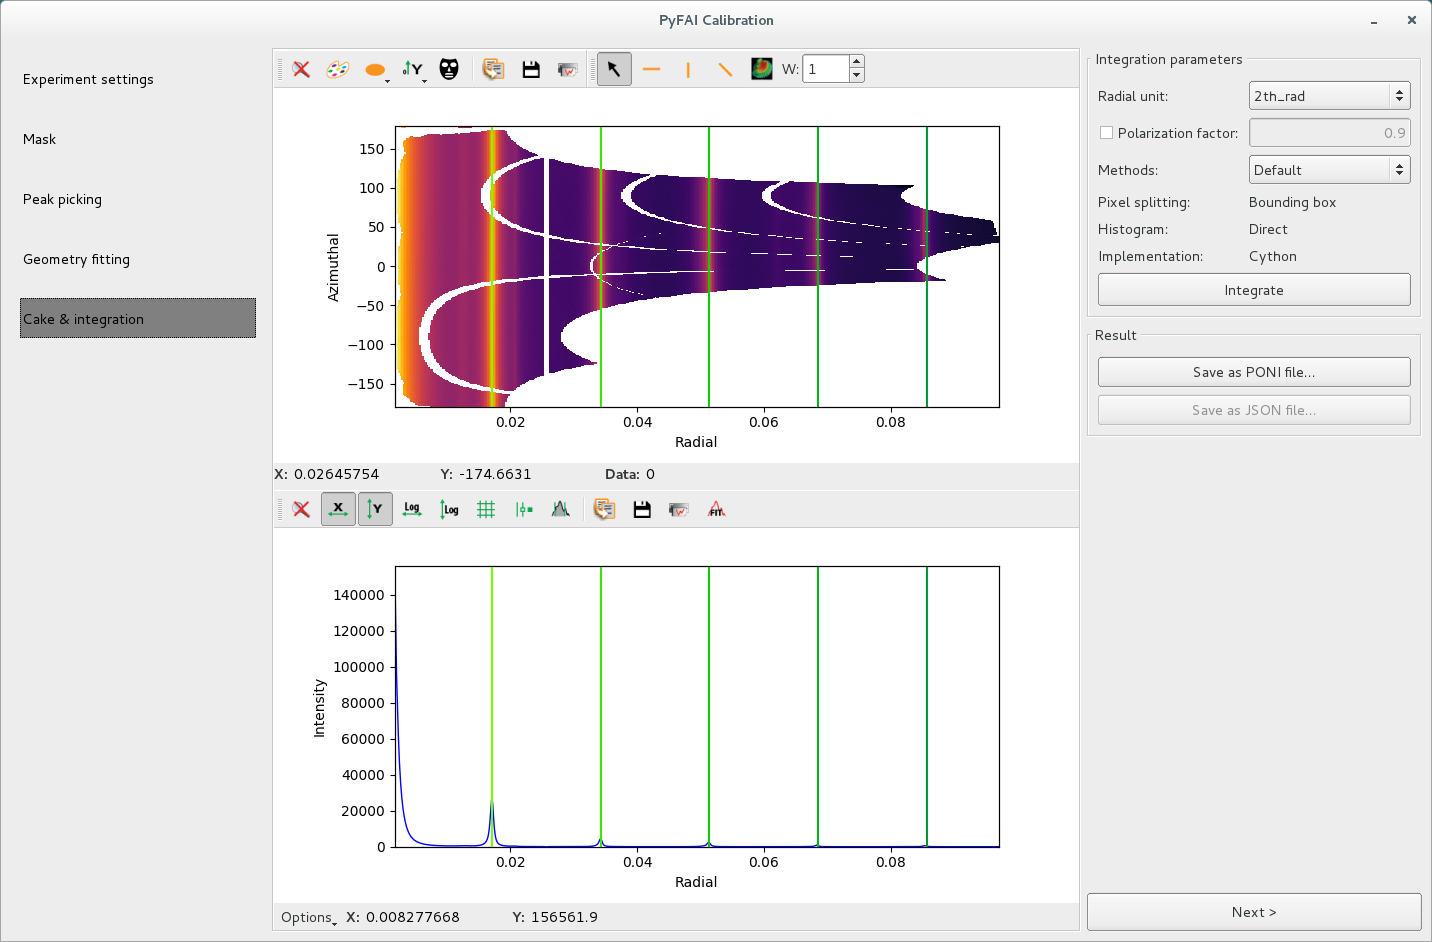
\includegraphics[width=9cm]{images/calibration-5-integration-result.png}
\caption{Integration interface to validate the geometry.}
\end{center}
\end{figure}


This new graphical user interface, while still under development, is already
available in the development branch of pyFAI and will be distributed in the
final version of pyFAI v0.14 to be release mid-2017.

\section{Calibration of a detector on a moving stage}

The calibration of the detector position on a fixed goniometer position can be
performed with pyFAI as long as the calibrant chosen leaves at least two rings
on the image and that five control-points can be extracted from one ring and
at least one point on the second ring. 
Of course, more points provides a better fit but this limit may be an issue
when dealing when very small area detectors are used (the ImXPad S10 is as
small as 80x120 pixels and it is still usable).

\subsection{Translation of geometry}

If the difficulty is not in the calibration, it is  rather in the variety of
goniometers and translation tables which may be controlled by one or multiple
motors.
Those motors are usually coupled with encoder, such as the actual position of
the motors is known precisely.
The goniometer implementation in pyFAI accepts an
arbitrary number of degrees of freedom for the goniometer which may be named 
(must be named for more than one degree of freedom). 
Let ($motor_1$, $motor_2$, \ldots, $motor_n$) be those motors. 

The work of calibrating the detector's arm is the to define a set of parameter
(of arbitrary size: $param_1$, $parma_2$, \ldots, $param_m$), the functions
$\Re$ which transforms them into the 6-parameters needed by pyFAI and the values
of the parameters such as for any position of the setup, this returns us a
proper geometry.

This can be expressed as:
$$
dist, poni_1, poni_2, rot_1, rot_2, rot_3 = \Re(param_1, param_2, \ldots,
param_m, motor_1, motor_2, \ldots, motor_n) 
$$

The 6 parameters contained in the \textsc{poni}-file  are then used to calculate
the $2\theta$ position of the peak positions which are compared to the expected $2\theta$
values calculated from the calibrant d-spacing and the wavelength. 
The sum of the square of those differences is used to minimize the parameter set
using the scipy.optimize.minimize function \cite{scipy}.

This translation function contains hence the motor names, the parameters names
and the six functions, one for each of the six parameters used in pyFAI. 

From a computer engineering perspective, it should also be serializable to 
disk (in \textsc{json}-format) to allow its restoration from a file without
having to re-perform the calibration. 
To address this constrain, the NumExpr software package \cite{numexpr} was
used, allowing the user to provide mathematical formula as text with an
arbitrary number of degrees of freedom for the goniometer and as many parameters
as needed.
The definition of this function is simply the instantiation of the
\textit{pyFAI.goniometer.GeometryTranslation} class, with a list of motor
names, parameter names and a set of six formula, one for each of the six parameters. 
This may appear complicated and is best explained by example.

\subsection{A simple example: the translation table}

At ESRF, protein crystallography beam-lines use large pixel-detectors (typically
Pilatus 6M from Dectris) placed on a translation stage which allows to collect
the data at the optimal distance: shorter detector distance for high-q and small
inter-reticular distances or longer distances for best spot separation.

PyFAI has the ``MX-calibrate'' tool available for calibrate many images taken at
various distances but this can be addressed as a goniometer setup: 

\begin{verbatim}
from pyFAI.goniometer import GeometryTranslation
gt = GeometryTranslation(param_names = ["dist_offset", "dist_scale", 
                                        "poni1", "poni2", "rot1","rot2"],
                         dist_expr="pos * dist_scale + dist_offset", 
                         poni1_expr="poni1",
                         poni2_expr="poni2", 
                         rot1_expr="rot1", 
                         rot2_expr="rot2", 
                         rot3_expr="0.0")
\end{verbatim}
 
In this example we define a 6-parameter set, most of them being exactly the same
as the one of pyFAI: $poni_1$, $poni_2$, $rot-1$ and $rot_2$. $rot_3$ is forced
to zero while the distance is defined a linear function of the motor position.
If no motor names are not provided, pyFAI assumes there is only one motor
called $pos$.

The Jupyter notebook \cite{ipython} in supplementary materials file
``TTcalibration'' presents the usage of this translation function together with
the translation table refinement. 
Initially this set of data has been calibrated using the ``MX-clibrate'' tool
which extracts automatically the control points from images taken at ESRF-MX
beam-lines from the metadata written in the header of images, so a good set
of control point has been available prior to the processing described. 
The translation table has been calibrated a first time with all control points
and this \textit{translation function} subsequently, all images have been
integrated azimuthally (Figure \ref{id29}, blue curve). 
The image is a zoom on the two first peaks which looks ``doubled'' indicating a
poor modeling of the geometry.

\begin{figure}
\label{id29}
\begin{center}
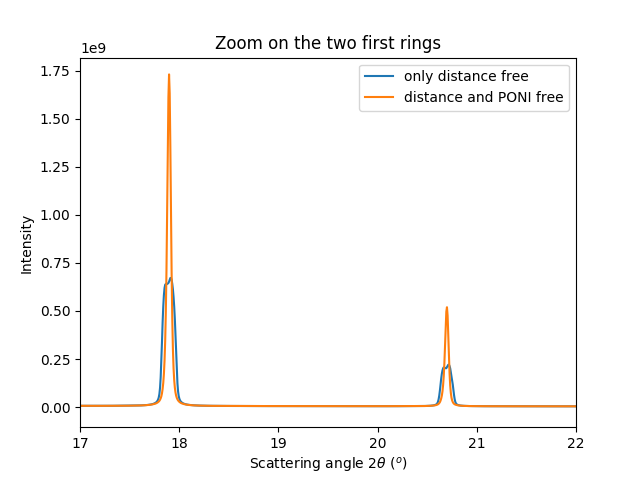
\includegraphics[width=9cm]{images/TranslationTable.png}
\caption{Powder diffraction profile obtained from seven images acquired
at various distances from 15 to 45 centimeters combined using a model with one
(distance) or 3 degrees of freedom (distance and detector center)}
\end{center}
\end{figure}


 
A second \textit{translation function} has been defined, allowing in addition a
linear dependency of the \textsc{poni} position with the detector distance and
the translation table model has been re-fitted (Figure \ref{id29}, orange
curve).
The peaks are much sharper, and the residual error is about $5\times$ smaller.
The residual error being the average over all control points of the deviation of
the $2\theta$ angle from theoretical value in radians, squared.

This example shows the \textsc{poni} is moving on the detector
plane by one millimeter per meter horizontally and four vertically.
This ``large'' vertical deviation has been confirmed by the beam-line staff and
is related to last focusing mirror, just before the sample, making the beam no
more horizontal.
Once everything is fitted, the quality of the geometry obtained is perfectly
suited for powder diffraction experiment and the resolution is of the order of
one pixel for any detector position.
  
\subsection{A more realistic example: a single axis goniometer}

Probably the main application of this work is to place a limited size detector
on a goniometer $2-\theta$ arm, which is described now.
In this second example, available as supplementary material file XXX, a single
Pilatus module (100k) is mounted on the arm which is moved from 5 to 65 degrees per half
degree step. 
So one hundreed and twenty one images of LaB6 calibrant has been acquired on the
ROBL beam-line (ESRF BM20, German CRG beam-line).
Due to the small size of the detector (487x197 pixels),
some of the images have no ring at all, most have one ring and only few images
have 2 rings.
The first images with two rings correspond to the rings of of the second group
of LaB6 and lay around angle of 30 to 35 degrees.
Three images, at 31.5, 33 and 35.5 degrees have been manually calibrated using
the pyFAI-calib tool.
This manual calibration is rather unstable due to the small size of the
detector. 
The rotation of the detector has been fixed to have consistency in the 3
calibration.

TODO

\section{Outlook}

This goniometer description can be adapted to many type of simple goniometer.
The \textit{TranslationFunction} class presented in the notebook may be extended
in the future to use the libhkl\cite{picca} which contains already many
diffractometers' geometries with their multiplication matrices. 
This is already possible but it won't allow the saving to and restoration from
file. 

By moving the detector in front of the sample, one can fill up the
gaps which exists in Pilatus detectors. Those gaps are known to be responsible for glitches
when acquiring PDF data with high energy photons due to the
polarization of the synchrotron beam, causing large anisotropy in the
diffracted signal.

Different generations of pixel detectctors have seen their pixel size
shrink:
from $\172 mu m$ for the Pilatus, $130 \mu m$ for ImXpad, $75 \mu m$ for the
Eiger and $55 \mu m$ for Medipix-based chips \ldots, and probably less for
future detectors.
As the resolution of the powder diffraction diagram obtained is limited by the
pixel size (and the distance of the detector), this shrinkage of pixel-size
leads naturally to better powder diffraction patterns. 
Unfortunatelly, to keep the surface of the detector contant, one would need
to increase the number of pixels by the square of this value, and the associated
infrastructure for read-out and data-transfer. 
By moving the detector in front of the sample, this limitation can partially be
removed.

\section{Conclusion}

The new graphical user interface for pyFAI has been developped to ease the
calibration of the experimental setup with fixed detector. 
On those fixed position have been described, they can be fitted togeather to
detemine the detector position at any position of the goniometer. 
By acquiring multiple images a variaous positions, images can be
integrated togeather to provide a powder diffraction pattern of
quality equivalent to the one acquired with a much larger detector. 

\bibliographystyle{iucr}
\bibliography{biblio}
 
\ack{Acknowledgements}

We would like to thank all ESRF beam-line teams for supporting the
pyFAI development, and especially David Flot from the MX-group who provided the
data of the translation table and the two CRG beamlines BM02 (D2AM) and BM20
(ROBL) for the goniometer data. 
They gracefully provided beam-time and test-data to allow debugging this 
goniometer optimization tool.
We would also like to thank the French CNRS for financing the IR-DRX project
in 2015 and 2016 which acted as a catalyzer on the goniometer refinement,
and the other participants to the project, especially Serge Cohen from the
Ipanema institute, the DiffAbs beamline and Frédéric-Emmanuel Picca from
Synchrotron Soleil.
In the instrumentation division (ISDD) we would like to thank V. A. Solé,  head
of data analysis unit and leader of the \textit{silx} project, and all our
colleagues from the silx project: Thomas Vincent, Henri Payno and Pierre Knobel.

\end{document}
